% This section has been adapted from the old moller manual
% and previous OSP/THA. wmhenry: Aug 2022

% Operations Manual Title



%\setcounter{subsection}{0}

\infolevone{
\chapter[M\o ller Polarimeter]{M\o ller Polarimeter 
\footnote{Author: W.Henry \email{wmhenry@jlab.org} adapted from the M{\o}ller manual written by J.Gomez}
}
}
\infolevone{
The Hall A M\o ller polarimeter is used to measure the polarization of the beam being delivered to Hall A.\footnote{(Home page: \textcolor{blue}{http://hallaweb.jlab.org/equipment/moller/})} 
This section provides an overview of the instrument and its operation as well as making the operators of this instrument aware of the hazards that this device presents. 
The system consists of (see Fig.\ref{fig:moller_layout}),
\vspace{-\parskip}
\begin{itemize}
\item  A magnetized ferromagnetic foil placed in the beam path. The foil acts as a polarized 
       electron target and it can be selected from a set of four different foils. The in-beam foil is magnetized by an adjustable field superconducting magnet. The foils are located 
       17.5~m upstream from the nominal 
       pivot point of the Hall A High Resolution Spectrometers.

\item A magnetic spectrometer system consisting of four quadrupole magnets and a dipole magnet. 
      The spectrometer focuses the electrons scattered in a particular kinematic
      range onto the M{\o}ller detector package.

\item A detector package and its associated shielding house.
\item Two stand-alone data acquisition systems.
\item An off-line analysis software package to extract the beam polarization. Roughly, 
      the beam polarization is calculated by taking the difference in the counting rates of
      two different beam helicity samples.
\end{itemize}
 
 \begin{figure}[ht]
    \begin{center}
        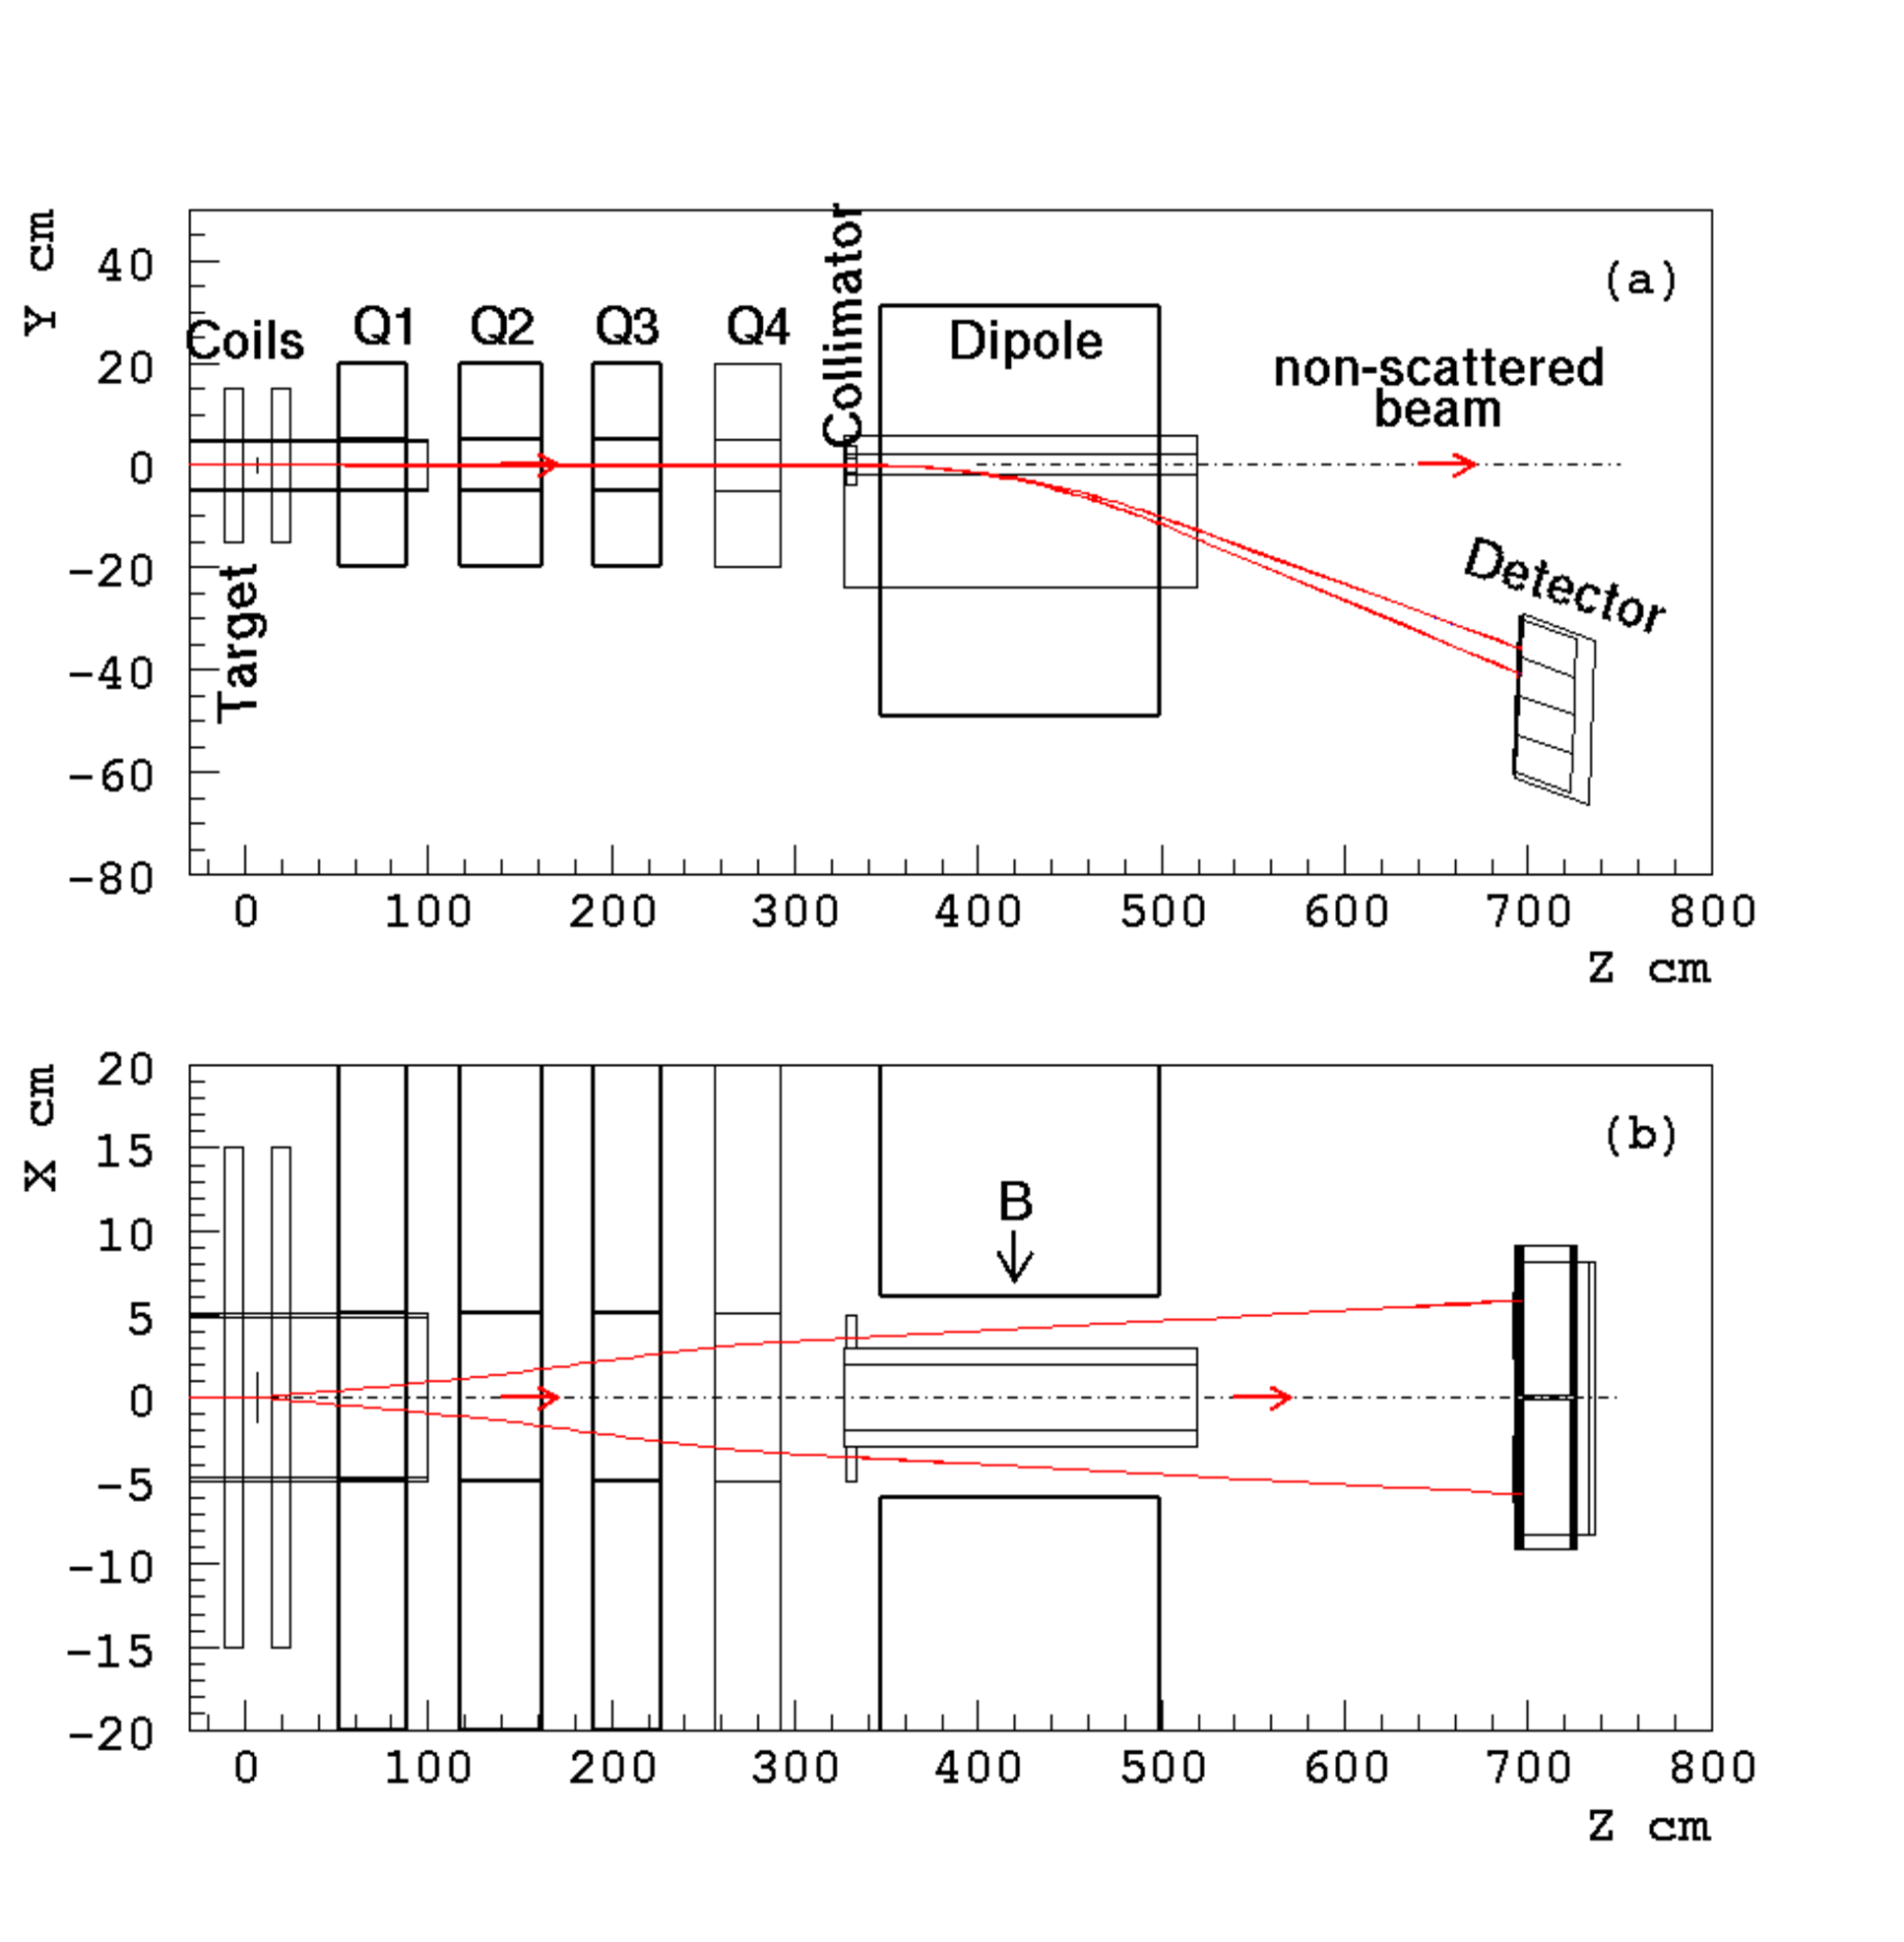
\includegraphics[angle=0,width=0.74\textwidth]{fig1}
    \caption[M{\o}ller: layout]{
            Layout of M{\o}ller polarimeter. The origin of the 
            coordinate frame is at the center of the polarimeter
            target, which is 17.5~m upstream of the Hall A target.
            }
    \label{fig:moller_layout} 
    \end{center}
 \end{figure}  
\section {Principles of Operation}
\label{sec:moller_principles}
\vspace{-\parskip}
The cross-section ($\sigma$) for M{\o}ller scattering 
$ \vec{e^-} + \vec{e^-} \rightarrow e^- + e^-$
depends on the beam and target polarizations ${\cal P}^{beam}$ and 
${\cal P}^{target}$ as:
$$         \sigma \propto 1 +  
            \sum_{i=X,Y,Z} (A_{ii}\cdot{}{\cal P}^{targ}_{i}\cdot{}{\cal P}^{beam}_{i}) $$
where $i = X,Y,Z$ defines the projections of the polarizations. 
The analyzing powers $A_{ii}$ depend on the scattering angle in the Center-of-Mass (CM) frame 
$\theta{}_{CM}$. 
Assuming that the beam direction is along the Z-axis and that the scattering
happens in the ZX plane of a right-handed Cartesian reference frame, then:
\begin{eqnarray*}
 A_{ZZ} &=&  -\frac{\sin^2\theta{}_{CM}\cdot(7+\cos^2\theta{}_{CM})}
                                   {(3+\cos^2\theta{}_{CM})^2}\ , \\
         A_{XX} &=& -\frac{\sin^4\theta{}_{CM}}
                       {(3 + \cos^2\theta{}_{CM})^2}\ , \\
         A_{YY} &=& -A_{XX}
\end{eqnarray*}

$A_{ZZ}$ is called the longitudinal analyzing power while $A_{XX}$ and $A_{YY}$ are referred to as the transverse analyzing powers.
The analyzing powers do not depend on the beam energy and they reach their maximum values when $\theta{}_{CM}=90^o$,
\begin{eqnarray*}
A_{ZZ}^{max} &=& 7/9\ ,\\
A_{XX}^{max} = - A_{YY}^{max} &=& A_{ZZ}^{max} / 7\ 
\end{eqnarray*}
The main purpose of the polarimeter is to measure the longitudinal component of the beam polarization.
The M{\o}ller polarimeter of Hall A detects pairs of scattered electrons in a 
range of $ 75^o < \theta{}_{CM} < 105^o$ with an average analyzing power 
of about $<A_{ZZ}>=0.76$.

The target consists of a thin magnetically saturated ferromagnetic foil.
In such a material, about 2 electrons per atom can be polarized.
The maximal electron polarization for fully saturated pure iron is 8.01\%.
In Hall A M{\o}ller polarimeter the foil is magnetized by a 3~T field parallel to the beam
axis and perpendicular to the foil plane.

The scattered electron pairs pass through a magnetic spectrometer
which selects particles in a particular kinematic region. Two electrons
are detected with a two-arm detector system and the 
coincidence counting rate of the two arms is measured.
The beam longitudinal polarization is then calculated as:
\begin{displaymath}
           {\cal P}^{beam}_{Z} = \frac{N_{+}-N_{-}}{N_{+}+N_{-}}\cdot{}
      \frac{1}{{\cal P}^{foil}\cdot{}<A_{ZZ}>},
\end{displaymath}
where $N_{+}$ and $N_{-}$ are the measured counting rates with two opposite
mutual orientation of the beam and target polarizations, while 
$<A_{ZZ}>$ is obtained using Monte-Carlo calculation of the M{\o}ller 
spectrometer acceptance. ${\cal P}^{foil}$ is derived from special
magnetization measurements in bulk material.

\section{Description of Components}

\vspace{-\parskip}

\subsection{Polarimeter Control}
\vspace{-\parskip}

Control of the M{\o}ller polarimeter is divided into two separate sections,
\vspace{-\parskip}
\begin{itemize}
\item The operators in the Machine Control Center (MCC) have sole control over the currents settings of the quadrupoles \& dipole that make up the magnetic spectrometer
of the polarimeter.
To access the Graphical User Interface (GUI)
screens used for control of the polarimeter,
\vspace{-\parskip}
\begin{itemize}
\item Launch \textcolor{blue}{NewTools} application located in any of the Hall A control computers.
\item Search for \textcolor{blue}{``Hall A Moller''} (keep quotes to do a phrase search)
\item Select \textcolor{blue}{Hall A Moller Combo} from the list. Fig.~\ref{fig:combo} shows the screen that will come up.
\end{itemize}
\item The user has control over the superconducting magnet current used to magnetically saturate
the in-beam target. See section \ref{SHC_sssection}.
\end{itemize}

   \begin{figure}%[htb]
      \begin{center}
          \includegraphics*[angle=-90,width=\textwidth]{moller/fig2}
      \end{center}
      \caption[M{\o}ller:MCC control screen]{The M{\o}ller MCC control screen.
            }
      \label{fig:combo} 
   \end{figure}  
\subsection{Polarized Electron Target }
\vspace{-\parskip}

Fig. \ref{fig:target} shows the M{\o}ller Polarized Electron Target. The target is
located on the beam line 17.5~m upstream of the main Hall A physics target and it consists of,
\vspace{-\parskip}
\begin{itemize}
  \item A split-coil, 5~T superconducting magnet with field oriented parallel to the beam (Z-axis)
  \item A target system with up to four (4) iron foils. The system moves along the vertical axis (Y-axis) to bring the foils in and out the beam path. The target system can also rotate the foils around the Y-axis.
        The foils are described on Table \ref{Tab1}.
\end{itemize}

\subsubsection{5T Magnet}
\label{SHC_sssection}
A cryogen-free, split coil, superconducting magnet from American Magnetics Inc. (AMI) is used to saturate the in-beam iron foil. Fig. \ref{fig:magnet} shows a drawing of the magnet system with relevant dimensions while
Fig. \ref{fig:specifications} shows the main characteristics of the magnet. To minimize stresses on the magnet that could induce a quench, field changes above 4.5~T proceed very slowly. While recovery from a magnet quench does not require operator intervention, it does take 36-48 hours for the magnet to reach back its operating temperature. To avoid waisting time while running experiments, the magnet has been set to be operated routinely up to 80 A ($\sim$ 4.28~T). A 3~T field is typically used to saturate the iron foils. 
 
   \begin{figure}%[ht]
      \begin{center}
         \includegraphics*[angle=0,width=0.55\textwidth]{moller/fig3}
      \end{center}
      \caption[M{\o}ller:target]{The M{\o}ller target area. The beam propagates from right to left.
            }
      \label{fig:target} 
   \end{figure}  

   \begin{figure}%[htb]
      \begin{center}
         \includegraphics*[angle=90,width=.8\textwidth]{moller/fig4}
      \end{center}
      \caption[High-field Target Magnet]{The 5~T target magnet from AMI. The electron beam travels along the 3-inch diameter warm bore of the magnet. The target system ladder moves in and out of the beam path along the vertical opening labeled RADIAL ACCESS on the drawing.}
      \label{fig:magnet} 
      \begin{center}
          \includegraphics*[angle=0,width=.7\textwidth]{moller/fig6}
      \end{center}
      \caption[PT415RM Pulsed-tube Cryogenic Refrigerator]{The various components of the 
               PT415RM pulsed-tube cryogenic refrigerator.}
      \label{fig:refrigirator} 
   \end{figure} 

\begin{figure}
\begin{minipage}[c]{0.6\linewidth}
\includegraphics*[width=\linewidth]{moller/fig5}
\caption[M{\o}ller target magnet specifications]{M{\o}ller target magnet specifications.}
 \label{fig:specifications} 
\end{minipage}
\hfill
\begin{minipage}[c]{0.3\linewidth}
\includegraphics*[width=\linewidth]{moller/fig7}
\caption[Advantage Engineering M1-3A water chiller]{An Advantage Engineering M1-3A water chiller provides the water cooling needed by the CP1110 compressor.}
 \label{fig:water_chiller} 
\end{minipage}%
\end{figure}
    

The magnet is conduction cooled by a pulse tube cryogenic refrigerator, model PT415-RM,  from CryoMech. The cryogenic refrigerator cold head is labeled PT CRYOCOOLER on Fig. \ref{fig:magnet}. 
Fig. \ref{fig:refrigirator} shows the various components of the cryogenic refrigerator.
Two 66~ft long flexible lines, a ``high-side'' and a ``low-side'', connect the compressor with the cold head. Two gauges on the compressor show the helium pressure on those lines. When the CP1110 compressor is not operating, the two gauges will show a pressure of $\sim$~220~psi. When the compressor begins operation and the cold head is at ambient temperature, the differential pressure between the high and low side lines is typically 220 to 250~psi. The differential pressure will decrease as the cold head cools down. If the high side pressure becomes larger than 360~psi, the compressor will trip. To reset the fault, the high side pressure needs to drop to 359~psi or below. The compressor is equipped with a over-pressure relief to atmosphere valve set at 420~$\pm$~5~PSIG. The cold head is equipped with a relief to atmosphere valve set to 425~$\pm$~5~PSIG. The total amount of helium in the system corresponds to $\sim$~850~liters NTP. 

An Advantage Engineering M1-3A water chiller (see Fig. \ref{fig:water_chiller}) provides the water cooling needed by the CP1110 compressor.
The M1-3A is an air cooled, 3 refrigeration-tons unit. The M1-3A and the CP1110 form a closed water circuit. Water temperature is set to 20$^\circ$~C (68$^\circ$~F).

Figure \ref{fig:cooldown_curves} shows the cool down curves for this magnet system.

   \begin{figure}%[htb]
      \begin{center}
          \includegraphics*[angle=0,width=0.8\textwidth]{moller/fig28}
      \end{center}
      \caption[Cool system down curves]{Magnet system cool down curves. Temperature sensor labels T1, T2, T6 and T7 correspond to those shown on Fig. \ref{fig:temperature_status}.}
      \label{fig:cooldown_curves} 
   \end{figure}  

Operation of the superconducting magnet and status of the supporting equipment is through various EPICS screens,
\vspace{-\parskip}
\begin{itemize}
\item Launch \textcolor{blue}{NewTools}.
\item Search for \textcolor{blue}{``Hall A Moller''} (keep quotes to do a phrase search)
\item Select \textcolor{blue}{Hall A Moller CP2800 Compressor} to see the status of the superconducting magnet cryogenic refrigeration system (Fig. \ref{fig:cryomech_status}). There are no user adjustable parameters in this system. Notify the primary contact (see Table \ref{Tab2}) if questions or problems arise with the cryogenic refrigerator or water chiller systems.
\item Select \textcolor{blue}{Hall A Moller Temperature} to see various temperatures around the superconducting magnet (Fig. \ref{fig:temperature_status}).
\item Select \textcolor{blue}{Hall A Moller Gaussmeter} to see the value of the ``witness field" measured by a Hall probe located next to the beam pipe, on the upstream flange of the magnet (Fig. \ref{fig:gaussmeter}). It is a simple cross-check that the magnet is operating as expected. \color{blue}This is not the magnetic field at the center of the split magnet where the target is located.\color{black}\ The measured relation between the ``witness'' gaussmeter and the superconducting magnet current is, 
\begin{displaymath}
B \sim 0.087\left({\rm kG \over A}\right)\ \times\ I
\end{displaymath}
%\vspace{-\parskip}
The sign of the ``witness'' field is the same than the magnet current. A positive field value means the magnetic field points downstream, towards the beam dump.
%shown on Table \ref{L20151210101744}.
\item Select \textcolor{blue}{Hall A Moller AM430 Power Supply} to operate \& monitor the magnet (Fig. \ref{fig:power_control}).
\end{itemize}

\begin{figure}
\begin{minipage}[c]{0.4\linewidth}
\includegraphics*[width=.7\linewidth]{moller/fig8}
\caption[CP1110 status]{CryoMech CP1110 refrigerator status.}
\label{fig:cryomech_status} 
\end{minipage}
\hfill
\begin{minipage}[c]{0.4\linewidth}
\includegraphics*[width=.7\linewidth]{moller/fig9}
\caption[Temperature status]{Magnet temperature status.}
 \label{fig:temperature_status} 
\end{minipage}%
\end{figure}

\begin{figure}
\begin{minipage}[c]{0.4\linewidth}
\includegraphics*[width=0.8\linewidth]{moller/fig11}
\caption[gaussmeter_reading]{Magnetic field measured by LakeShore Hall Probe.}
\label{fig:gaussmeter} 
\end{minipage}
\hfill
\begin{minipage}[c]{0.4\linewidth}
\includegraphics*[width=.8\linewidth]{moller/fig10}
\caption[Moller magnet supply]{Control and operation of the magnet.}
 \label{fig:power_control} 
\end{minipage}%
\end{figure}

Before operating the magnet, check that the magnet temperatures (see Fig. \ref{fig:temperature_status}) shown by the Lakeshore temperature measurement unit are close to those shown on Table \ref{temperature_start}.
If they are, bring up the magnet power supply GUI (see Fig. \ref{fig:power_control}) and follow the sequence to operate,
\begin{table}[htb]
\begin{center}
\begin{tabular}{| p{6cm} | p{2cm} |} \hline
Temperature Sensor   & \hfill $^\circ$ K \\
\hline 
  Cryocooler (T1)   &  \hfill  3.3 - 3.7 \\
  Magnet (T2) & \hfill 3.8 \\
  Magnet Lead \#1 (T6)  &  \hfill 43   \\
  Magnet Lead \#2 (T7)  &   \hfill 42   \\
\hline
\end{tabular}
\end{center}
\caption[Magnet temperatures in the superconducting state]{Magnet temperatures in the superconducting state with no current flowing through the magnet.}
\label{temperature_start}
\end{table}

\vspace{-\parskip}
\begin{enumerate}
\item If \textcolor{blue}{Persistance Heater Control} switch is \textcolor{blue}{OFF} (indicated by red frame around \textcolor{blue}{OFF} button), press switch \textcolor{blue}{ON}. A message will appear next to \textcolor{blue}{Ramp State} indicating the heater is being turned on. The button frame will change color (green) and move to the \textcolor{blue}{ON} button. Wait for the heater message to disappear before proceeding to change the magnet current.
\item The \textcolor{blue}{Ramp State} shows the current state of the supply,
\vspace{-\parskip}
\begin{itemize}
\item \textcolor{blue}{Paused} indicates the supply output current is being kept constant at the value it had when the \textcolor{blue}{Ramp Control - Pause} switch was pressed.
\item A message along the lines of \textcolor{blue}{``Holding at target"} indicates the supply output current is the value requested under \textcolor{blue}{Current Target}.
\item A message along the lines of \textcolor{blue}{``Ramping to target"} indicates the supply output current is ramping at pre-programmed rates towards the \textcolor{blue}{Current Target} value.
\end{itemize}
\item Enter the \textcolor{blue}{Current Target} based on the field desired (0.536 kG/Amp). Positive values will produce a magnetic field directed downstream towards the beam dump. The variable \textcolor{blue}{Current} shows the actual current circulating in the magnet. If the new \textcolor{blue}{Current Target} has opposite polarity than that shown by \textcolor{blue}{Current}, the supply will automatically ramp first to 0, reverse its polarity and then ramp up to the new requested current. \textcolor{red}{Do not exceed $\pm$ 80 A.}
\item If the \textcolor{blue}{Ramp State} is \textcolor{blue}{Paused}, the supply will not change the magnet current until the \textcolor{blue}{Ramp Control - Ramp} switch is pressed. Pressing \textcolor{blue}{Ramp Control - Pause}, will prevent the supply from changing its output current. If the \textcolor{blue}{Ramp State} was ``holding" when a new \textcolor{blue}{Current Target} value was entered, the power supply would have started automatically to ramp towards the new value.
\item The voltage across the magnet leads is shown under \textcolor{blue}{Voltage}. \textcolor{blue}{Field} shows the calculated field at the center of the magnet based on the value of \textcolor{blue}{Current}.
\item When the current reaches the set value, a message will appear next to \textcolor{blue}{Ramp State} indicating that the supply is ``holding'' at target. The voltage across the magnet leads will drop to 0. Proceed with measurements.
\item When finished performing measurements:
\vspace{-\parskip}
\begin{enumerate}
\item Set \textcolor{blue}{Current Target} to 0;
\item Wait until \textcolor{blue}{Current} reaches 0, then turn \textcolor{blue}{OFF} the \textcolor{blue}{Persistance Heater Control} switch. A message will appear next to the \textcolor{blue}{Ramp State} indicating the heater is cooling. The button frame will change color (red) and move to the \textcolor{blue}{OFF} button. It takes quite a bit longer to turn off the heater than to turn it on.\hfill\break
\textcolor{red}{NOTE:} If the persistance switch is turned off before the magnet current reaches zero, there will be a magnetic field in the magnet which may interfere with beam delivery.
\end{enumerate}
\end{enumerate}

If a magnet quench occurs, the message next to \textcolor{blue}{Quench?} in the power supply GUI (Fig. \ref{fig:power_control}) will become \textcolor{red}{QUENCH!!} otherwise the message \textcolor{blue}{OK} will be displayed. \textcolor{blue}{Count} indicates the total number of quenches detected by the magnet power supply since it was brought into operation at the factory. If a quench occurs, the magnet current will drop to 0 and all the temperatures shown on the magnet temperatures GUI (Fig. \ref{fig:temperature_status}) will increase substantially.
An estimate of how long will take to re-cool the magnet and be able to operate it again can be made by comparing those temperatures with the cool down curves shown on Fig. \ref{fig:cooldown_curves}. \color{blue}Before leaving the magnet to re-cool, perform the following steps, in the order shown, to reset the supply and turn off the persistance heater,\color{black}\ 
\vspace{-\parskip}
\begin{enumerate}
\item Press \textcolor{blue}{Clear} on the power supply GUI  to reset the quench condition
\item Turn off the \textcolor{blue}{Persistance Heater Control}
\end{enumerate}

The magnet power supply is located in the Hall A corridor leading to Hall A. It is an 4Q06125PS-430 from AMI.
The maximum voltage across the magnet leads when ramping is 1 V (3 V across the power supply terminals). The current is limited to a maximum of $\pm$ 80 A. 
Use the provided external ``witness''
gaussmeter (see Fig. \ref{fig:gaussmeter}) to determine that the field is ramping and its orientation. Recall that this meter does not measure the field at the center of the magnet but at a convenient location outside the magnet.
\subsubsection{M{\o}ller Target Foils}
Figures \ref{fig:targetonstand} and \ref{fig:foils} show a general view of the target system and a close up of the target ladder itself.
Operation of the target system is through the screen shown in
Fig.~\ref{fig:target_control}. To get to it, either press the blue button next to the label \textcolor{blue}{Target Motion Control} in
Fig. ~\ref{fig:combo} or by searching for \textcolor{blue}{``Moller Target Control"} after launching \textcolor{blue}{NewTools}.


\begin{figure}
\begin{minipage}[c]{0.45\linewidth}
          \includegraphics*[width=0.95\linewidth]{moller/fig14}
      \caption[Target control screen]{Target motion/rotation control screen.}
      \label{fig:target_control} 
\end{minipage}
\hfill
\begin{minipage}[c]{0.45\linewidth}
     \includegraphics*[width=.55\linewidth]{moller/fig12}
 \caption[Target System]{Target system. The target ladder can be seen at the bottom of the system.}
\label{fig:targetonstand} 
\end{minipage}%
      \begin{center}
\includegraphics*[angle=0,width=.35\textwidth]{moller/fig13}
\caption[Target ladder detail]{Target lader with foils.}
 \label{fig:foils} 
      \end{center}
   \end{figure}  

 
\begin{table}[htb]
\begin{center}
\begin{tabular}{| p{3cm} | p{3cm} | p{1.5cm} | p{1.5cm} | p{1.5cm} | p{1.5cm} |} \hline
          & \multicolumn{5}{|c|}{Position} \\ \cline{2-6}
          & \hfill 0  &  \hfill 1  &   \hfill  2  &   \hfill  3   &   \hfill  4   \\
%          &   &     &     &      &      \\
%          &  Limit  &     &     &      &      \\
\hline 
  Material            &  \hfill  none &  \hfill none &  \hfill Fe &  \hfill Fe &  \hfill Fe \\
  Purity (\%) & - & \hfill - & \hfill 99.99 & \hfill 99.99 & \hfill 99.85 \\
  Thickness ($\mu$m)   &  \hfill  -    &  \hfill -  &   \hfill 10   &  \hfill 4  &  \hfill 1   \\
  Polarization (\%)      &        \hfill  -   &  \hfill - &  \hfill 8.01 &  \hfill 8.01 &  \hfill 8.01 \\
  Comment             &  Retracted target position &        &        &      &    \\
%                                &  position  &        &        &        &     \\
\hline
\end{tabular}
\end{center}
\caption[Moller target foils]{Target foil parameters. Purity and thickness are as quoted by manufacturer, Goodfellow Corporation. An ``Extended Limit'' stops the motion
of the target slider a short distance past foil\#~4 and the FSD interlock will not allow
for beam delivery. In the ``Retracted Target Position'' (Position 0), the edge of the target ladder is several
inches away from the beam.}
\label{Tab1}
\end{table}

The target ladder (see Fig. \ref{fig:foils}) can be moved vertically, placing different foils
into the beam. The whole target ladder can also be rotated around the Y-axis 
in an angle range $\sim\pm 6.5^\circ$.

The MCC operator must {\bf ``mask''} the M{\o}ller target motion before performing any target motion.
Authorized Hall A personnel (see section~\ref{sec:moller-pers}) are also allowed to move the target. 

Three closed-circuit TV cameras, located in the Hall A Counting House, are used to observe the target motion. One camera looks from the side and shows the angular orientation of the target to the beam and two limit switches corrsponding the target angle $-6.5^\circ$ and $+6.8^\circ$ accordingly. The second camera shows 
the vertical position of the target rail. The third camera looks from the bottom of the magnet camera through the window and shows the target loader inside the magnet.

Data Acquisition ``dead time'' typically limits the beam current that can be used to perform a beam polarization measurement to about 1.0~$\mu$A while
localized beam heating of the iron foils (which causes some loss of target polarization) would limit the beam currents to less than 2~$\mu$A.

M{\o}ller target position interlocks, used to indicate when the various targets are properly located in the beam path, are routed to the Fast ShutDown 
(FSD) system of the accelerator. Fig.~\ref{fig:moller_fsd} shows the crate which controls
the signals. The M{\o}ller FSD crate is located in Hall A rack 02. Target control is via EPICS (ref) Input \& Output Controller (IOC) {\bf IOCHLA}.  The master section of this IOC is located in the corridor leading to Hall A, in the bottom of rack 1H75L05 (see Fig.~\ref{fig:moller_ioc}). The slave crate with the field wirings is located in Hall A rack 02 
 below the M{\o}ller FSD crates (see Fig.~\ref{fig:moller_fsd}).
\
   \begin{figure}%[htb]
      \begin{center}
          \includegraphics*[angle=0,width=0.7\textwidth]{moller/fig15}
      \end{center}
      \caption[M{\o}ller: FSD crate.]{The M{\o}ller target
            motion may cause the Fast ShutDown (FSD) of the accelerator.
            The LEDs in the top right corner show the appropriate
            signals from the target. The top LED lit indicates
            no FSD signal. 
            }
      \label{fig:moller_fsd} 
   \end{figure}  

 
   \begin{figure}%[htb]
      \begin{center}
          \includegraphics*[angle=0,width=0.6\textwidth]{moller/fig16}
      \end{center}
      \caption{EPICS IOC {\bf IOCHLA} master 
               crate is located in the corridor leading to Hall A in the bottom of rack 1H75L05. 
            }
      \label{fig:moller_ioc} 
   \end{figure}  
\subsection {Spectrometer Description }
\label{sec:moller_compon_spectr}
\vspace{-\parskip}
The M{\o}ller polarimeter spectrometer consists of four quadrupole magnets and one
 dipole magnet. Fig.\ref{fig:spectrometer} shows a side view
 of the spectrometer,
\vspace{-\parskip}
\begin{list}{$\bullet$}{\setlength{\itemsep}{-0.10cm}}
   \item quadrupole {\bf MQM1H02A} (white color, there is no label on the yoke);
   \item quadrupole {\bf MQM1H02} (red color, on the yoke labeled {\bf $PATSY$});
   \item quadrupole {\bf MQO1H03} (blue color, on the yoke labeled {\bf $TESSA$}); 
   \item quadrupole {\bf MQO1H03A} (blue color, on the yoke labeled {\bf $FELICIA$})
   \item dipole {\bf MMA1H01} (on the yoke marked as {\bf $University \, of \,
    Kentucky$}).
\end{list} 
\vspace{-\parskip}
All of these magnetic elements are controlled by MCC operators since they can steer the beam. 

%\noindent
   \begin{figure}%[htb]
      \begin{center}
          \includegraphics*[angle=0,width=0.8\textwidth]{moller/fig17}
      \end{center}
      \caption[M{\o}ller:spectrometer]{The M{\o}ller spectrometer. The target is located at the right
            side of the photograph.
            }
      \label{fig:spectrometer} 
   \end{figure}  

The spectrometer accepts electrons scattered close to the horizontal 
plane (see Fig.\ref{fig:moller_layout}). The acceptance in the azimuthal
angle is limited by a collimator in front of the dipole magnet, while
the detector vertical size and the magnetic field in the dipole magnet limit 
the acceptance in the scattering angle $\theta_{CM}$.

The electrons have to pass through the beam pipe in the 
region of the quads, through the collimator in front of 
the dipole magnet, with a slit of 0-4~cm high, through two vertical
slits in the dipole, about 2~cm wide, positioned at $\pm$4~cm 
from the beam. These slits are terminated with vacuum tight windows
at the end of the dipole. The dipole deflects the scattered 
electrons down, towards the detector. The detector, consisting
of 2 arms - 2 vertical columns - is positioned such that electrons, 
scattered at $\theta_{CM}=90^o$ pass close to its center. 
This acceptance is about $76<\theta_{CM}<104^o$. At beam energies below 1~GeV
the vertical slits in the dipole limit the acceptance to about
$83<\theta_{CM}<97^o$.

Energy range of the spectrometer is 1.0~GeV $\div$ 11.0~GeV. For a given beam 
energy there is an optimal setting of the currents in these 5 magnets. 

Typically, the dipole magnet should be turned on
only for the M{\o}ller measurements. 
\subsection {Detector}
\label{sec:moller_compon_det}
\vspace{-\parskip}
The M{\o}ller polarimeter detector is located in the shielding box downstream 
of the dipole and consists of two identical modules placed symmetrically about a 
vertical plane containing the beam axis, thus enabling coincidence measurements 
(see Fig.~\ref{fig:moller_detector}). Each part of the detector includes:
\vspace{-\parskip}
\begin{itemize}
 \item An aperture detector consists of four scintillators with light guides and 
       Hamamatsu R4124 (13~mm diameter) photomultiplier tubes connected to each segment. 
       Size of the aperture assembled detector is 31$\times$4$\times$3.8~cm.
  \item A {\it spaghetti} lead - scintillating fiber calorimeter\footnote{
         before summer 2002 a lead glass calorimeter consisting of 48~$\times$8$\times$~30~cm$^3$
         was used. It lost a big fraction of the amplitude due
         to the radiation damage and deterioration of the optical contact.},
         consisting of 2 blocks \\
         9$\times$15$\times$30~cm$^3$, each separated into 2
         channels equipped with Photonis XP2282B (2~inch) photomultiplier tubes. Thus,
         each of the vertical detectors is segmented into 4 calorimeter channels.
\end{itemize}

   \begin{figure}%[htb]
      \begin{center}
          \includegraphics*[angle=0,width=0.7\textwidth]{moller/fig18}
      \end{center}
      \caption[M{\o}ller:detector]{The M{\o}ller detector in the shielding box. 
               The aperture detector on the face of the lead - scintillating fiber 
               calorimeter is not shown. 
            }
      \label{fig:moller_detector} 
   \end{figure}  

 The HV crate is located in Hall A behind the decommissioned LHRS on the second platform behind the dipole  (see. Fig.~\ref{fig:moller_hv}). 
 The HV is controlled by a GUI located in JMENU (see Fig.~\ref{fig:mollerHVgui}).
 HV for the various calorimeter blocks is tuned in order to align the M{\o}ller peak
 position at a ADC channel 300 for each module.

   \begin{figure}%[htb]
      \begin{center}
          \includegraphics*[angle=0,width=0.7\textwidth]{moller/fig19.jpg}
      \end{center}
      \caption[M{\o}ller:HV]{The M{\o}ller HV crate (CAEN 5527 Crate with three AG7236 HV cards.  Slot 1 is positive HV used for the Compton and slots 3,4 are negative HV cards).}
      \label{fig:moller_hv} 
   \end{figure}

   \begin{figure}%[htb]
      \begin{center}
          \includegraphics*[angle=0,width=0.9\textwidth]{moller/fig19b.png}
      \end{center}
      \caption[M{\o}ller:HV]{The M{\o}ller HV GUI located in jmenu.
            }
      \label{fig:mollerHVgui} 
   \end{figure}     

\subsection {Electronics}
\label{sec:moller_compon_ele}
\vspace{-\parskip}
 The electronics, used for M{\o}ller polarimetry, is located
 in several crates in the Hall (racks 12, 14, 15):
\vspace{-\parskip}
\begin{list}{}{\setlength{\itemsep}{-0.15cm}}
  \item[1.] VME, board computer {\bf hallavme5} - for DAQ;
  \item[2.] CAMAC - for the trigger and data handling;
  \item[3.] NIM - for the trigger and data handling;
  \item[4.] LeCroy~1450 - HV crate, slots {\bf 5} and {\bf 6}
            (calorimeter and aperture detector).
\end{list}
\noindent
   The photograph on Fig.~\ref{fig:electronics} shows (from left to right) the 
   DAQ crates in rack 14, power supplies for the M{\o}ler spectrometer quadrupole 
   magnets in rack 13 and FADC DAQ crates in rack 12. Rack 14 from the top to bottom: 
   crate with delay lines (blue), two M{\o}ller target Helmholtz coils power supplies. 
   Crate below the power supplies is the VME DAQ crate and Helmholtz coils control, 
   the next one is the CAMAC crate and the bottom one is the NIM crate.

   \begin{figure}%[hbt]
      \begin{center}
          \includegraphics*[angle=0,height=0.8\textheight]{moller/fig20}
      \end{center}
      \caption [M{\o}ller:electronics crates.] {M{\o}ller electronics, located
             in the Hall, at the right side of the beam line. From left to right:
             the DAQ crates in rack 14, power supplies for the M{\o}ler 
             spectrometer quadrupole magnets in rack 13 and FADC DAQ crates in rack 12.
            }
      \label{fig:electronics} 
   \end{figure}  

%\noindent
One can connect to the CPU boards and the HV crate via a portserver:
\vspace{-\parskip}
\begin{list}{}{\setlength{\itemsep}{-0.15cm}}
  \item[1.] {\bf hallavme5}~ - {\bf hatsv5} port {\bf 4};
  \item[4.] LeCroy 1450 - {\bf hatsv5} port {\bf 3}.
\end{list}

\subsection {DAQ}
\label{sec:moller_compon_daq}
\vspace{-\parskip}
Two data acquisition (DAQ) systems in are used. The original DAQ%
\footnote{(More details in: 
\textcolor{blue}{http://hallaweb.jlab.org/equipment/moller/guide1.2\_linux.html})} 
 is based on CODA~\cite{CODAwww} and runs on {\it adaq2}.
 The database server for CODA is running on {\it adaq1}. A more recent DAQ system, still undergoing evaluation, is based on Flash Analogue-to-Digital Converters (FADC) in VME format. This system runs on the {\it hamoller} computer and it uses Portserver {\it hatsv12 port 5} to connect to the VME modules.
Data is stored on 
{\it hamoller:/data1/raw/}. The FADC DAQ 
 electronics is located in the Hall rack 12 (see Fig.~\ref{fig:fadc}).
 
   \begin{figure}%[htb]
      \begin{center}
          \includegraphics*[angle=0,width=0.8\textwidth]{moller/fig21}
      \end{center}
      \caption[M{\o}ller:fadc]{The M{\o}ller FADC crates.
            }
      \label{fig:fadc} 
   \end{figure}  

\subsection {Slow Control}
\label{sec:moller_compon_slow}
\vspace{-\parskip}
The Helmholtz coils are controlled via a script starting automatically
at the beginning of each CODA run. The polarity of the current in the coils
is reversed at every new run.

The HV, the electronics settings and the collimator position
are controlled from a Java program with a GUI%
\footnote{More details in \textcolor{blue}{http://hallaweb.jlab.org/equipment/moller/slow\_mpc.html}}.

Procedure to start the slow control task,
\vspace{-\parskip}
 \begin{list}{--}{\setlength{\itemsep}{-0.15cm}}
   \item Login to {\it adaq1} as {\it moller};
   \item {\it adaq1$>$~cd~Java/msetting/}
   \item {\it adaq1$>$~./mpc} \ \ \ $\Leftarrow$ it starts the slow control task.
 \end{list}
\vspace{-\parskip}
 It may take about a minute to start all the components and read out
 the proper data from the electronic crates.

  The slow control GUI is presented on Fig.~\ref{fig:slow_control}.
   \begin{figure}[htb]
      \begin{center}
          \includegraphics*[angle=0,width=0.8\textwidth]{moller/fig22}
      \end{center}
      \caption[M{\o}ller:slow control window]{The slow control GUI (Java).
            }
      \label{fig:slow_control} 
   \end{figure}  

 The components are: 
\vspace{-\parskip}
 \begin{list}{--}{\setlength{\itemsep}{-0.15cm}}
   \item \textcolor{blue}{EPICS~\cite{EPICSwww} Monitor}: these EPICS variables are stored for every DAQ run
   \item \textcolor{blue}{Detector Settings} is used to set up the thresholds, delays etc.
   \item \textcolor{blue}{High Voltage Control} for the photomultiplier tubes
   \item \textcolor{blue}{Motor Control} to move the collimator
   \item \textcolor{blue}{Target Monitor} information on the target position, magnets etc.
 \end{list}

  High voltage can be changed or turned on/off using the HV GUI window 
  (Fig.~\ref{fig:hv_gui}), where the first eight channels belong to the calorimeter 
  and the other eight channels belong to the aperture counters.
   \begin{figure}[htb]
      \begin{center}
          \includegraphics*[angle=0,width=0.8\textwidth]{moller/fig23}
      \end{center}
      \caption[M{\o}ller:HV control]{HV control GUI window.
            }
      \label{fig:hv_gui} 
   \end{figure}  

  The settings of the CAMAC electronics used to select the trigger
  and control DAQ are controlled using the \textcolor{blue}{Detector Setting} window 
  (Fig.~\ref{fig:detector_gui}):
\vspace{-\parskip}
   \begin{list}{--}{\setlength{\itemsep}{-0.15cm}}
     \item \textcolor{blue}{Delay line} - the delays for the calorimeter and aperture counter signals;
     \item \textcolor{blue}{LedDiscriminator} - discriminator thresholds for the calorimeter and the counters
     \item \textcolor{blue}{PLU Module} - settings of the logical unit
   \end{list}
\vspace{-\parskip}

   \begin{figure}[htb]
      \begin{center}
          \includegraphics*[angle=0,scale=0.4]{moller/fig24}
      \end{center}
      \caption[M{\o}ller: electronics control]{Detector setting GUI window.
            }
      \label{fig:detector_gui} 
   \end{figure}  

  The collimator width can be changed using
  \textcolor{blue}{Motor Control} window (Fig.~\ref{fig:motor_gui}).
  
   \begin{figure}%[htb]
      \begin{center}
          \includegraphics*[angle=0,scale=0.3]{moller/fig25}
      \end{center}
      \caption[M{\o}ller: collimator control]{GUI window to control the dipole 
               collimator size (and also the slide, which is not relevant here).
            }
      \label{fig:motor_gui} 
   \end{figure}  
\section {Operating Procedure }
\label{sec:moller_oper}
\vspace{-\parskip}

The procedure includes general steps as follows: 
\vspace{-\parskip}
\begin{list}{$\bullet$}{\setlength{\itemsep}{-0.15cm}}
  \item ``Non-invasive'' preparations - start the appropriate
          computer processes, turn on the HV and learn the
          magnet settings needed;
  \item ``Invasive'' preparations: beam tuning with the regular
          magnet settings, loading the M{\o}ller settings,
          beam tuning, if neccessary, installing the M{\o}ller target;
  \item Detector check/tuning;
  \item Measurements;
  \item Restoring the regular settings.
\end{list}
The ``non-invasive'' preparations can be done without disturbing the running 
program in the Hall. It is reasonable to perform these preparations
before starting the ``invasive'' part.

In more details, the ``invasive'' procedure looks as follows:
\vspace{-\parskip}
 \begin{list}{--}{\setlength{\itemsep}{-0.15cm}}
   \item Remove the main target;
   \item Load the M{\o}ller settings in the magnets, keep the dipole off; 
   \item Tune the beam position with any convenient beam current;
   \item Turn on the M{\o}ller dipole; 
   \item Check the beam position;
   \item Tune the beam to $\sim{}0.5~\mu$A for M{\o}ller measurements; 
   \item Pull in the M{\o}ller target, using the TV camera to make sure the foil is at the
         window center;
   \item Take CODA run;
 \end{list}
\subsection {Initialization}
\label{sec:moller_oper_initial}
\vspace{-\parskip}
In order to control the operations, several terminal sessions
of the {\bf moller} account must be opened on {\bf adaq1,...}.
The data analysis and some initial calculations are done using a PAW~\cite{PAWwww}
session on  {\bf adaq1}:
%\vspace{-\parskip}
 \begin{list}{--}{\setlength{\itemsep}{-0.15cm}}
   \item Login to {\bf adaq1} as {\bf moller};
   \item {\bf adaq1$>$~cd~paw/moller}, start PAW (type {\bf paw}), select Workstation type 3.  
 \end{list}
\noindent
\vspace{-\parskip}
Check that the portserver connections are available:
%\vspace{-\parskip}
 \begin{list}{--}{\setlength{\itemsep}{-0.15cm}}
   \item Try {\bf telnet hatsv5 2003} and {\bf telnet hatsv5 2004};
   \item If a connection is refused - clean it up, by connecting
         {\bf telnet hatsv5} as root and typing {\bf kill 3} or {\bf kill 4},
         see instructions in {\bf $\sim$adaq/doc/portserver.doc}.    
 \end{list}
\noindent
\vspace{-\parskip}
Slow control:
%\vspace{-\parskip}
 \begin{list}{--}{\setlength{\itemsep}{-0.15cm}}
   \item Login to {\bf adaq1} as {\bf moller};
   \item Start the slow control (see section~\ref{sec:moller_compon_slow});
   \item Load the regular settings and the appropriate HV.
 \end{list}
\noindent
\vspace{-\parskip}
CODA runs on {\bf adaq1}: 
%\vspace{-\parskip}
 \begin{list}{--}{\setlength{\itemsep}{-0.15cm}}
   \item Login to {\bf adaq1} as {\bf moller}, make two sessions;
   \item {\bf adaq2$>$ kcoda} - clean up the old coda;
   \item Reset the VME board {\bf hallavme5} by: {\bf telnet hatsv5 2004}, {\bf -$>$ reboot};  
%   \item {\bf adaq2$>$ et\_start moller \&} - start ET if it is not running;
%   \item Reset {\bf hallavme5} and {\bf halladaq14} by pressing two top left green
%         reset buttons in the middle room of the counting house;
   \item {\bf adaq2$>$ start\_coda} - start CODA;
   \item Click {\bf Connect} and select the configuration {\bf beam\_pol};
   \item Click {\bf Download} to download the program into the VME board.
 \end{list}
\subsection {Initial Beam Tune}
\label{sec:moller_oper_initbeam}
\vspace{-\parskip}

 Typically, the M{\o}ller measurements are taken during the regular Hall A
 running, when the beam has been tuned for this running. However,
 the M{\o}ller measurements require a different magnetic setting.
 At least the dipole magnet has to be turned on. This magnet
 slightly deflects the beam downward. The deflection at the main target
 could be $<3$~mm, depending on the beam energy. It is, therefore, 
 useful to tune the beam position before the dipole is turned on. It can be done
 before the magnets are set to the M{\o}ller mode.
 The requirements for straight beam are: 
\vspace{-\parskip}
 \begin{list}{--}{\setlength{\itemsep}{-0.15cm}}
   \item On BPM IPM1H01 (in front of the M{\o}ller target) $|X|<0.1$~mm, $|Y|<0.1$~mm.
   \item On BPM IPM1H04 (downstream of the M{\o}ller detector)  $|X|<0.1$~mm, $|Y|<0.1$~mm.
%   \item On BPM IPM1C20 (upstrean of the Compton chicane)  $|X|<0.1$~mm, $|Y|<0.1$~mm.
 \end{list}
\vspace{-\parskip}
 These requirements should be given to MCC.
\subsection {The Magnet Settings}
\label{sec:moller_oper_magset}
\vspace{-\parskip}

The proper M{\o}ller magnets (quads and dipole) settings for the given beam energy 
have to be providet to MCC by the M{\o}ller polarimeter team.\footnote{A reasonable accuracy in the  magnets settings is about 1-2\%.}
%\begin{safetyen}{5}{2}
%\color{red}
   The beam must be turned off when the magnets are being tuned. 
 %\end{safetyen}
% \color{black}

\subsection {Final Beam Tune}
\label{sec:moller_oper_finalbeam}
\vspace{-\parskip}
 The beam parameters for M{\o}ller measurements
 are: 
 \vspace{-\parskip}
  \begin{list}{--}{\setlength{\itemsep}{-0.15cm}}        
     \item 
     %\begin{safetyen}{5}{0} 
   %  \color{red}
     beam currents between $\sim{}0.5~\mu$A and $<2~\mu$A;
      %\end{safetyen}
%      \color{black}
     \item the beam current should be reduced mainly by closing the ``slit''
           in the injector (not by the laser attenuator), in order to
           reduce the effect of current leak-through from the other halls.
   \end{list}
\
\subsection {Target Motion}
\label{sec:moller_oper_target}
\vspace{-\parskip}
 The procedure is as follows:
% MCC should be asked to: %put in one of the targets (typically, the {\bf bottom}
\vspace{-\parskip}
   \begin{list}{--}{\setlength{\itemsep}{-0.15cm}}        
     \item Ask the MCC to mask the main target (cryotarget or whatever) motion
           and remove the main target, then ask the MCC to unmask the motion;
     \item Ask the MCC to mask the M{\o}ller target motion;
     \item Move to target to the position needed (say, 4) using
           the MEDM screen {(see Fig.~\ref{fig:target_control})}.
           Check that the target is close to the center of the window
           in the TV camera screen. 
   \end{list}

\subsection{Detector Tuning and Checking }
\label{sec:dettune}
\vspace{-\parskip}

The goal is to check that the detector is working, that the counting rates
are normal and that the M{\o}ller peaks are located at about ADC channel 300
for all the calorimeter blocks.

\vspace{-\parskip}
\begin{list}{}{\setlength{\itemsep}{0.5cm}}
  \item[A.] Data taking with CODA
  \vspace{-\parskip}
      \begin{list}{}{\setlength{\itemsep}{0.cm}}
             \item[1.] Take a RUN for about 20k events. Let us assume the run 
                       number is 9911.
        \end{list}
  \item[B.] Data analysis with PAW
\vspace{-\parskip}
        \begin{list}{--}{\setlength{\itemsep}{0.cm}}
             \item[1.]  {\bf PAW$>$~exec~run~run=9911}: build an NTUPLE and 
                       attach it to the PAW session;
             \item[2.]  {\bf PAW$>$~exec~lg\_spectra~icut=60~run=9911}: look at the 
                       ADC distributions. The peaks should be at about ADC channel 300
                       for all 8 modules. If the peaks are off - try to adjust
                       the HV (do not go beyond 1990V).
        \end{list}
  \item[C.] Check of the background
\vspace{-\parskip}
        \begin{list}{}{\setlength{\itemsep}{0.cm}}
             \item[1.] Raise the thresholds to 240~mV of the channels 1 and 2
                       of the discriminator, using the slow control window 
                       (see section~\ref{sec:moller_compon_slow});
             \item[2.] Take a run of about 20k events, say run=9915;
             \item[3.]  {\bf PAW$>$~exec~lg\_spectra~icut=60~cut=11~run=9915}: look at the 
                       ADC distributions. The peaks should be at about ADC channel 300
                       for all 8 modules. The histograms 9 and 10 present the sums
                       of the left and right arms.
                       The histogram 11 (sum of both arms) should contain a clean peak at
                       about channel 600;
             \item[4.] {\bf PAW$>$~exec~asymu~run=9915}: polarization analysis should
                       provide a reasonable number. Check the scaler rates per second.
                       The counting rates in each arm should not exceed 600kHz. If they
                       are higher ask the MCC to reduce the beam current.
        \end{list}
\end{list}
\subsection {Polarization Measurement }
\label{sec:polmeas}
\vspace{-\parskip}

\begin{list}{$\bullet$}{\setlength{\itemsep}{0.cm}}
  \item[1.] Take an even (say, 2) number  of runs of data, each run of about 20-30~k
            events (30~k at $E_{beam}<2$~GeV).
  \item[2.] Analyze the data
\vspace{-\parskip}
        \begin{list}{--}{\setlength{\itemsep}{0.cm}}
             \item[1.] {\bf PAW$>$~exec~run~run=$Run\_Number$} and
             \item[2.] {\bf PAW$>$~exec~asymu~run=$Run\_Number$}, for each RUN,
        \end{list}
\end{list}
\subsection {Polarization Measurement with FADC}
\label{sec:polmeas_fadc}
\vspace{-\parskip}

   ROOT\cite{ROOTcern} based analyzer is used to process data from FADC DAQ.
   Data analysis is performed on {\bf hamoller} computer under ``a-onl'' 
   account. One should go to directory 
   {\bf moller$\backslash$moller$\_$fadc-18Feb2011$\backslash$} 
   and type command: \\
   {\bf a-onl$>$~source~root-setup.sh} \\
   Move into the analysis directory: \\
   {\bf a-onl$>$~cd~onlana} \\
   To replay a new run ($<Run\_Number>$) and generate a new .root file: \\
   {\bf a-onl$>$~analyzer}  \\
   In analyzer terminal type: \\
   {\bf ROOT$>$~replay$\_$test($<Run\_Number>$)} \\
   To analyse run ($<Nevents>$ is number of events to analyze, -1 - all events)
   type: \\
   {\bf ROOT$>$~$t=T(<Run\_Number>$)} \\
   {\bf ROOT$>$~$t->Loop(<Nevents>$)} \\
   Few graphic windows will be pop up and calculated asymmetries are printed
   in analyzer terminal.

}
\begin{safetyen}{0}{0}
\infolevone{\section{Safety Information}}
\infoleveqnull{\section{M\o ller Polarimeter}}
%
% Information for the ESAD
%
\label{sec:moller_safety}
\vspace{-\parskip}

\subsection{Hazards}
There are several specific hazards (potentially beyond those found in
the accelerator beamline) associated with the M\o ller Polarimeter.
These include:
\begin{enumerate}
\item{{\bf Radiation areas:} These are potentially caused by use of the M\o ller using thick targets, at higher than normal currents, or at low energies.}
\item{{\bf Magnets:}
\vspace{-\parskip}
Particular care must be taken in working in the vicinity of the magnetic elements of the polarimeter as they can have largecurrents running in them. The power supply (62~V, 500~A rating) for the dipole is located in the Beam Switch yard Building(Building 98). The maximum current for the dipole is 450A. The power supplies for quadrupoles {\bf MQM1H02}, {\bf MQO1H03}and {\bf MQO1H03A} (40~V, 330~A rating) are located in Hall A electronics rack 13 
\infolevone{
(see Fig.~\ref{fig:electronics})
}
. The power supply for quadrupole {\bf MQM1H02A} is 
located behind the Hall A electronics racks 
\infolevone{
(see Fig.~\ref{fig:quad_ps})
}
.
The status of the quadrupole power supplies is on the  checklist for closing up Hall A. 



\infolevone{
   \begin{figure}[htb]
      \begin{center}
          \includegraphics*[angle=0,width=0.8\textwidth]{moller/fig26}
      \end{center}
      \caption[M{\o}ller:magnet on]{``MAGNET ON'' light panel on the top of 
              the M{\o}ller spectrometer shielding guard.
            }
      \label{fig:magnet_on} 
   \end{figure}  
}

\infolevone{
   \begin{figure}[htb]
      \begin{center}
          \includegraphics*[angle=0,width=0.7\textwidth]{moller/fig27}
      \end{center}
      \caption[M{\o}ller:quad power supply]{Power supply for the M{\o}ller quadrupole 
              magnet {\bf MQM1H02A} locates in the Hall A.
            }
      \label{fig:quad_ps} 
   \end{figure}  
}



}
\item{{\bf Vacuum Windows:}
One must be careful in working near the downstream side of the dipole
magnet, as there are two 2 by 16~cm, 4~mil thick titanium windows.
}
\item{{\bf High Voltage:}
There are 16 photomultiplier tubes within the detector shielding hut, with a maximum voltage of 3000~V. The detector is serviced by sliding it back on movable rails. 
}
\item{{\bf Target:}
To avoid damage to the M{\o}ller target, the target should not be in the beam 
if the beam current is greater than 5$\mu$A. 
}
\item{{\bf Lead:}
The detectors are shielded using painted lead bricks.
}
\end{enumerate}
\subsection{Mitigations}
The special hazards associated with the Hall A M\o ller are mitigated as
described below.
\begin{enumerate}
\item{{\bf Radiation Areas:} Potential radiation areas are surveyed and posted before access to the hall is permitted after beam operations.}
\item{{\bf Magnets:} The quadrupole magnets and the leads for the dipole magnet are protected with Plexiglas shields. 
Removal of these shields requires following JLab's ``Lock out / Tag out'' procedure and ESH\&Q rules.
Concurrence from the Hall A work Coordinator must be obtained before proceeding with such work. 

As with all elements of the polarimeter which can affect the beamline, the magnets 
are controlled by MCC. There is a light panel ``MAGNET ON'' 
\infolevone{(see Fig.~\ref{fig:magnet_on})}
which indicates the status of the M{\o}ller polarimeter magnets (quadrupole magnets 
{\bf MQM1H02A}, {\bf MQM1H02}, {\bf MQO1H03}, {\bf MQO1H03A} and dipole magnet 
{\bf MMA1H01}).The light panel is placed on the top of M{\o}ller magnets plastic 
shielding box and lighting when any one of the M{\o}ller magnets is energized.

}
\item{{\bf Vacuum Windows:}
The windows are partially protected by a lead collimator downstream
of the dipole. Only members of the M{\o}ller polarimeter group should work 
in this area. If work is done on the collimators, the appropriate ear
and eye protection should be used.
}
\item{{\bf High Voltage:}
The high voltage must be turned
off during any detector movement. Only members of the M{\o}ller group should move the detector.
The M{\o}ller detectors use standard SHV connectors. }
\item{{\bf Target:}
Operation restrictions prevent beam greater than 5$\mu$A.  When the M{\o}ller target is in the beam line only authorized personal will communicate with MCC.  The experimenters are responsible for ensuring that the M{\o}ller target is 
removed from the beam for regular running and that its position is unmasked.  Additionally, the target motion system has a FSD to prevent the target being in the beam line during normal running.   
}
        \item{{\bf Lead:} Before removing lead bricks to access detectors, contact the JLab Industrial Hygiene group to mitigate any possible lead exposure.
}
\end{enumerate}

\infolevone{
\section{Authorized  Personnel}
}
\infoleveqnull{
\subsection{Authorized  Personnel}
}
\label{sec:moller-pers}
\vspace{-\parskip}
The list
of the presently authorized personnel is given in Table \ref{Tab2}.
Other individuals must notify and receive permission from
the contact person before adding their names 
to the above list.
%\obsolete{
\begin{table}[ht]
\begin{center}
\begin{tabular}{|ll|c|l|l|c|} \hline
  \multicolumn{2}{|c|}{Name} & Dept. & Ext. & 
  \multicolumn{1}{c|}{e-mail} & Comment \\ 
%  \cline{4-5}
 %  &  &   & JLab & Pager &  & \\ 
\hline
Donald & Jones & JLab &  7434 & jonesdc@jlab.org & Primary Contact \\
Dave & Gaskell & JLab &  6092 & gaskelld@jlab.org & \\
Ellen & Becker  & JLab    & 6436 & ebecker@jlab.org      &     \\
%  Oleksandr    & Glamazdin       & Kharkov & 5441 & glamazdi@jlab.org &  \\ 
%  Javier & Gomez  & JLab    & 7498 & gomez@jlab.org      &      \\ 
  William & Henry & JLab &  6929 & wmhenry@jlab.org & \\

%  Simona & Malace  & JLab    & 5289 & simona @jlab.org      &      \\
  Eric & King  & Temple   & - & ericking @jlab.org      &     \\
%  Charles & Clark  & Temple   & - & cpclark@jlab.org      &      \\    
%  Jim & Napolitano & Temple U. & - & tuf43817@temple.edu &  \\
%Viktor       & Gorbenko        & Kharkov & 5441 & gorbenko@jlab.org &  \\ 
% Roman        & Pomatsalyuk     & Kharkov & 5395 & romanip@jlab.org  &  \\ 
% Vadym       & Vereshchaka     & Kharkov & 5441 & vadym@jlab.org    &  \\
%   James & Wilhelmi & Temple U. & - & wilhejames@gmail.com & - \\
\hline
\end{tabular}
\end{center}
\caption[Moller Polarimeter: authorized personnel]{
   Moller Polarimeter: authorized personnel.
}
\label{Tab2}
\end{table}
\end{safetyen}
